\underline{Interferencja} jest to zjawisko powstawania nowego, przestrzennego rozkładu amplitudy fali (wzmocnienia i wygaszenia) w wyniku nakładania się (superpozycji fal) dwóch lub więcej fal. Warunkiem trwałej interferencji fal jest ich spójność, czyli korelacja faz i równość częstotliwości. 

Dla najprostszego przypadku dwóch fal harmonicznych o jednakowych amplitudach A, jednakowej długości fali $ \lambda $ i zgodnych fazach początkowych, rozchodzących się z dwóch różnych źródeł, które leżą w odległościach odpowiednio $ d_1 $ i $ d_2 $ od punktu P, zaburzenie w punkcie P opisuje wzór:\newline
$ y(P) = A\sin (\omega t + \phi_1) + A\sin (\omega t + \phi_2)$, gdzie:\newline
$ \phi_1 = 2\pi\frac{d_1}{\lambda} $,\newline
$ \phi_2 = 2\pi\frac{d_2}{\lambda} $.\newline
Gdy spełniony jest warunek:\newline
$ \phi_1 - \phi_2 = 2\pi\frac{d_1-d_2}{\lambda} = 2k\pi $,\newline
gdzie k - dowolna liczba naturalna, to fale w punkcie P ulegają wzmocnieniu (są w tej samej fazie) i:\newline
$ y(P) = 2A\sin (\omega t) $.\newline
Gdy natomiast w pewnym punkcie $ P_1 $:\newline
$ \phi_1 - \phi_2 = 2\pi\frac{d_1-d_2}{\lambda} = (2k+1)\pi $\newline
wtedy fale wygaszają się (są w przeciwfazie) i:\newline
$ y(P_1) = 0 $.

Interferencja pozwala na bardzo precyzyjny pomiar zmian długości drogi od źródła do detektora fali.

\underline{Dyfrakcja} (ugięcie fali) – zespół zjawisk związanych ze zmianą kierunku rozchodzenia się fali będący odstępstwem od praw optyki geometrycznej (dział optyki zajmujący się wytłumaczeniem zjawisk optycznych przy użyciu pojęcia promienia). Dyfrakcję w węższym znaczeniu określa się jako ugięcie światła wokół krawędzi przeszkody lub otworu w obszarze cienia przeszkody.

Zjawisko dyfrakcji rozpatruje się jako interferencję fal cząstkowych powstających zgodnie z zasadą Huygensa. Jest to zasada stosowana do określenia rozchodzenia się fali w ośrodku, mówiąca, iż każdy punkt ośrodka, do którego dotarło czoło fali, można uważać za źródło nowej fali kulistej. Wypadkową powierzchnię falową tworzy powierzchnia styczna do wszystkich powierzchni fal cząstkowych i ją właśnie obserwuje się w ośrodku.

Rysunek~\ref{diffracion} przedstawia dyfrakcję na pojedynczej szczelinie. Gdy różnica dróg fali ze skrajnego i środkowego elementu równa jest połowie długości fali, to fale z obu połówek szczeliny wygaszą się. Jeżeli wiązki są niemal równoległe, to różnica odległości pojawia się tylko przy wyjściu promieni ze szczeliny, wówczas:\newline
$ d\sin(\theta_{min}) = \lambda $.\newline

Przepuszczenie fali przez szczelinę dyfrakcyjną pozwala na określenie kierunku rozchodzenia się fali. Im mniejsza jest szerokość szczeliny, tym dokładniej można to zrobić. Jednocześnie zmniejszanie szczeliny powoduje, że trudniej jest określić energię fali, ponieważ rozprasza się ona na większy obszar. W efekcie iloczyn błędu określenia energii oraz błędu pomiaru kierunku musi być większy od pewnej stałej. Oznacza to, że istnieje granica dokładności pomiaru parametrów rozchodzącej się fali. Próba dokładniejszego określenia jednego z parametrów fali powoduje zwiększenie niepewności pomiaru drugiego sprzężonego z nim. Zjawisko to ma fundamentalne znaczenie, jeżeli weźmie się pod uwagę, że każda materialna cząstka jest falą. Zjawisko to w mechanice kwantowej odpowiada zasadzie nieoznaczoności

\begin{figure} [H]
	\centering
	\begin{subfigure}{.99\textwidth}
		\centering
		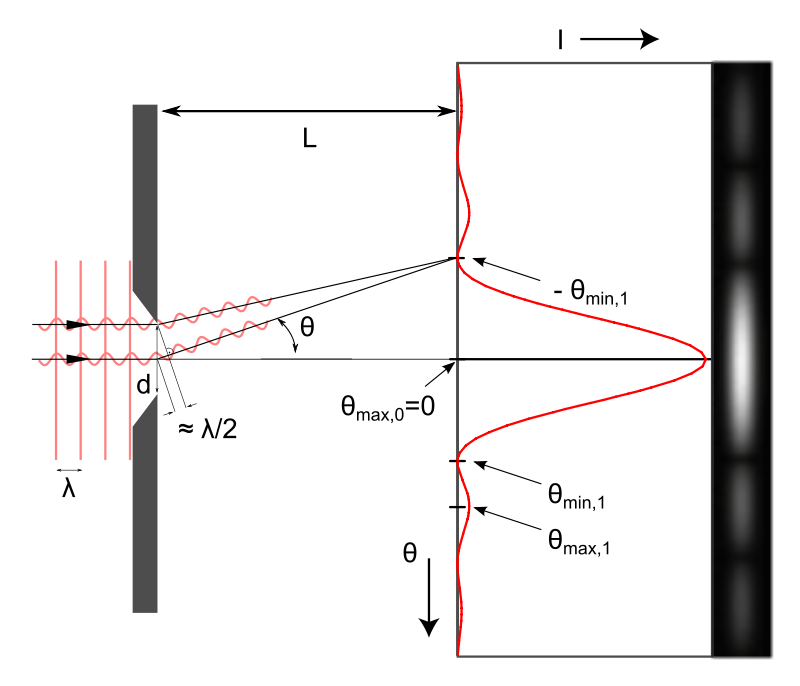
\includegraphics[width=0.6\linewidth]{generalIssues/Figures/diffraction.png}
	\end{subfigure}
	\caption{Dyfrakcja na pojedynczej szczelinie.}
	\label{diffracion}
\end{figure}

Pierwszą najprostszą formę eksperymentu przejścia światła przez podwójną szczelinę (rysunek~\ref{diffracion2}), zwaną obecnie doświadczenie Younga wykonał Thomas Young w 1801 roku. Eksperyment ten był zaczątkiem do uznania w XIX w falowej teorii światła. 

\begin{figure} [H]
	\centering
	\begin{subfigure}{.99\textwidth}
		\centering
		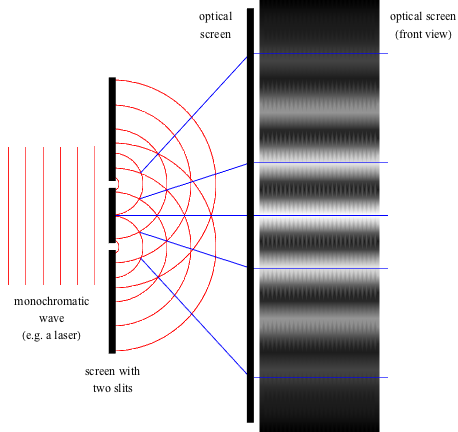
\includegraphics[width=0.6\linewidth]{generalIssues/Figures/diffraction2.png}
	\end{subfigure}
	\caption{Przejście światła przez podwójną szczelinę.}
	\label{diffracion2}
\end{figure}

Dla obrazów dyfrakcyjnych powstałych po przejściu światła przez otwór kołowy definiuje się \underline{warunek Rayleigha} określający zdolność rozdzielczą elementów i układów optycznych:\newline
$ \phi \approx \sin(\phi) = 1.22 \frac{\lambda}{d} $ (przybliżenie dla małych kątów), gdzie:\newline
$ \phi $ - minimalny kąt między promieniami, których obrazy mają być rozróżnialne, czyli inaczej – ich odległość kątowa,\newline
$ \lambda $ - długość fali światła,\newline
$ d $ - średnica otworu.\newline

Aby wzmocnić falę przechodzącą przez szczelinę stosuje się w optyce układy wielu takich szczelin, nazywane \underline{siatką dyfrakcyjną} (rysunek~\ref{diffracion3}). Efekty optyczne od każdej szczeliny dodają się, przez co zachowanie fali zależy tylko od stałej siatki (odległości dzielącej najbliższe sobie rysy). Zjawisko dyfrakcji zachodzi również, kiedy fale przechodzą przez wiele blisko siebie położonych warstw. Jeżeli odległość między warstwami jest stała, kolejne maksima fali można opisać zależnością:\newline
$ \sin(\theta) = \frac{n\lambda}{d} $, gdzie:\newline
$ d $ - stała siatki,\newline
$ \theta $ - kąt od osi wiązki światła,\newline
$ \lambda $ - długość fali,\newline
$ d $ - przyjmuje wartości całkowite dodatnie od 1,2,3,...\newline

\begin{figure} [H]
	\centering
	\begin{subfigure}{.99\textwidth}
		\centering
		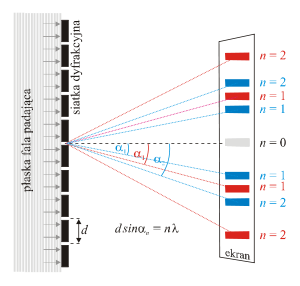
\includegraphics[width=0.6\linewidth]{generalIssues/Figures/diffraction3.png}
	\end{subfigure}
	\caption{Siatka dyfrakcyjna.}
	\label{diffracion3}
\end{figure}

Zjawisko dyfrakcji pozwoliło na rozwój krystalografii rentgenowskiej, dzięki której badano strukturę kryształów, odkryto w ten sposób także strukturę spirali DNA. 